\section{Μοντελοποίηση - ορισμός αεροελαστικών εξισώσεων}

Με το μοντέλο που περιγράφηκε παραπάνω, θα εξάγουμε τις αεροελαστικές εξισώσεις που περιγράφουν την κίνηση της αεροτομής. Οι εξισώσεις διατυπώνονται για τη γενική περίπτωση που έχουμε ελαστική σύζευξη, που ισχύει όταν έχουμε μη-μηδενική γωνία $\theta$. Θεωρώντας δεδομένα την ελαστικότητα (σταθερές ελατηρίων), τη γωνία της αεροτομής, και τη γωνία προσβολής του ανέμου, εφαρμόζωντας την ενεργειακή μέθοδο Lagrange, οι ελαστικές εξισώσεις προκύπτουν ως:

\begin{equation}
   \begin{aligned} 
    m\ddot{u} + \big(cos^2\theta\cdot k_{\xi} + sin^2\theta \cdot k_{\zeta}\big)\cdot u + sin\theta cos\theta\cdot (k_{\zeta}-k_{\xi})\cdot w &= F_x\\
    m\ddot{w} + sin\theta cos\theta (k_{\zeta}-k_{\xi})\cdot u + \big(sin^2\theta\cdot k_{\xi} + cos^2\theta \cdot k_{\zeta}\big)\cdot w  &= F_z\\
   \end{aligned} 
    \label{eq:genElastic}
\end{equation}

Ή μητρωϊκά, 

\begin{equation}
   \underbrace{
   \begin{bmatrix} 
   m & 0\\ 0 & m
   \end{bmatrix}
   }_{\mathbf{M}}
   \begin{Bmatrix}
   \ddot{u} \\ \ddot{w}
   \end{Bmatrix} 
   +
   \underbrace{
   \begin{bmatrix}
    cos^2\theta\cdot k_{\xi} + sin^2\theta \cdot k_{\zeta}\big & sin\theta cos\theta\cdot (k_{\zeta}-k_{\xi})\\
    sin\theta cos\theta\cdot (k_{\zeta}-k_{\xi}) & sin^2\theta\cdot k_{\xi} + cos^2\theta \cdot k_{\zeta}\big)
   \end{bmatrix}
   }_{\mathbf{K}}
   \begin{Bmatrix}
   u\\ w
   \end{Bmatrix} 
   = 
   \begin{Bmatrix}
   F_x\\ F_z
   \end{Bmatrix} 
    \label{eq:matElastic}
\end{equation}

Με βάση την εξίσωση \ref{eq:matElastic}, σημειώνονται τα εξής. Το μητρώο K αφορά το μετασχηματισμένο μητρώο δυσκαμψίας της αεροτομής απο το τοπικό της σύστημα στο γενικό. Επίσης, οι εξισώσεις \ref{eq:genElastic}, \ref{eq:matElastic} βρίσκονται στην πρωτογενή τους μορφή. Δηλαδή, δεν μπορούμε να ποσοτικοποιήσουμε την επίδραση της αεροδυναμικής στην απόσβεση απο την εξίσωση \ref{eq:matElastic}.

Αν γραμμικοποιήσουμε την εξίσωση \ref{eq:matElastic} γύρω απο μια θέση (έστω τη θέση ισορροπίας), τότε παίρνει την παρακάτω μορφή (εξ. \ref{eq:linAeroel}).

\begin{equation}
    [\mathbf{M}]\delta\ddot{\mathbf{u}} + 
    \underbrace{
    \begin{bmatrix}
    -\dpart{F_x}{\dot{u}} & -\dpart{F_x}{\dot{w}}\\[8pt]
    -\dpart{F_z}{\dot{u}} & -\dpart{F_z}{\dot{w}}
    \end{bmatrix}
    }_{\mathbf{C}}
    \delta\dot{\mathbf{u}} + [\mathbf{K}]\delta\mathbf{u} = 
    \mathbf{F}_0 -[\mathbf{M}]\ddot{\mathbf{u_0}} - [\mathbf{K}]\mathbf{u_0}
    \label{eq:linAeroel}
\end{equation}

Η μορφή της εξίσωσης \ref{eq:linAeroel} είναι πολύ χρήσιμη στην ιδιοανυσματική ανάλυση, απο όπου μπορούμε να εξάγουμε πληροφορίες για την ευστάθεια της αεροτομής μέσω του λόγου απόσβεσης. Φυσικά, η εξίσωση \ref{eq:linAeroel} μας παρέχει πληροφορία για την ευστάθεια στο σημείο γραμμικοποίησης, δηλαδή, αν γραμμικοποιήσουμε σε σημείο κοντά αλλά πριν την αντιστροφή της κλίσης του διαγράμματος $Cl-\alpha$ (βλ. σχήμα \ref{fig:cl}), η αεροτομή θα φανεί πιθανότατα ευσταθής, παρ'όλο που κατά την ταλάντωσή της μπορεί να βρεθεί σε σημείο όπου έχουμε αρνητική απόσβεση, και σε αυτό θα αναφερθούμε σε επόμενες παραγράφους.

Οπότε, πλέον, με αφετηρία την εξίσωση \ref{eq:genElastic} ή \ref{eq:matElastic}, μπορούμε να καθορίσουμε τις αεροελαστικές εξισώσεις για μόνιμη και μη-μόνιμη ροή.

\subsection{Αεροελαστικές εξισώσεις μόνιμης ροής}

Σε αυτή την περίπτωση, θα υπολογίσουμε την άνωση και την αντίσταση χρησιμοποιώντας δεδομένα για αεροτομή που προκύπτουν απο μόνιμη πλήρως ανεπτυγμένη ροή. Για την υλοποίηση της εργασίας, χρησιμοποιήσαμε αεροτομή NACA 2412, και προσεγγίσαμε τις  καμπύλες $Cl-\alpha, Cd-\alpha$ χρησιμοποιώντας προσομοίωση με συνεκτική ροή στο XFOIL. Στο λογισμικό που αναπτύχθηκε, έγινε προεκβολή για τιμές εκτός του εύρους της προσομοίωσης, με ανάπτυγμα Taylor χρησιμοποιώντας όρους δεύτερης τάξης, και θέσαμε όριο στις $\pm50^o$ για να αποφύγουμε την αύξηση του σφάλματος για μεγάλες τιμές της γωνίας προσβολής. Για γωνίες μεταξύ αποτελεσμάτων των προσομοιώσεων, οι τιμές των $Cl, Cd$ λαμβάνονται με γραμμική παρεμβολή. Τέλος, οι τιμές της κλίσης, λαμβάνονται με κεντρικές πεπερασμένες διαφορές. Οι καμπύλες $Cl, Cd$ που προκύπτουν φαίνονται στα διαγράμματα \ref{fig:cl}, \ref{fig:cd}.

\begin{figure}[ht!]
    \begin{center}
        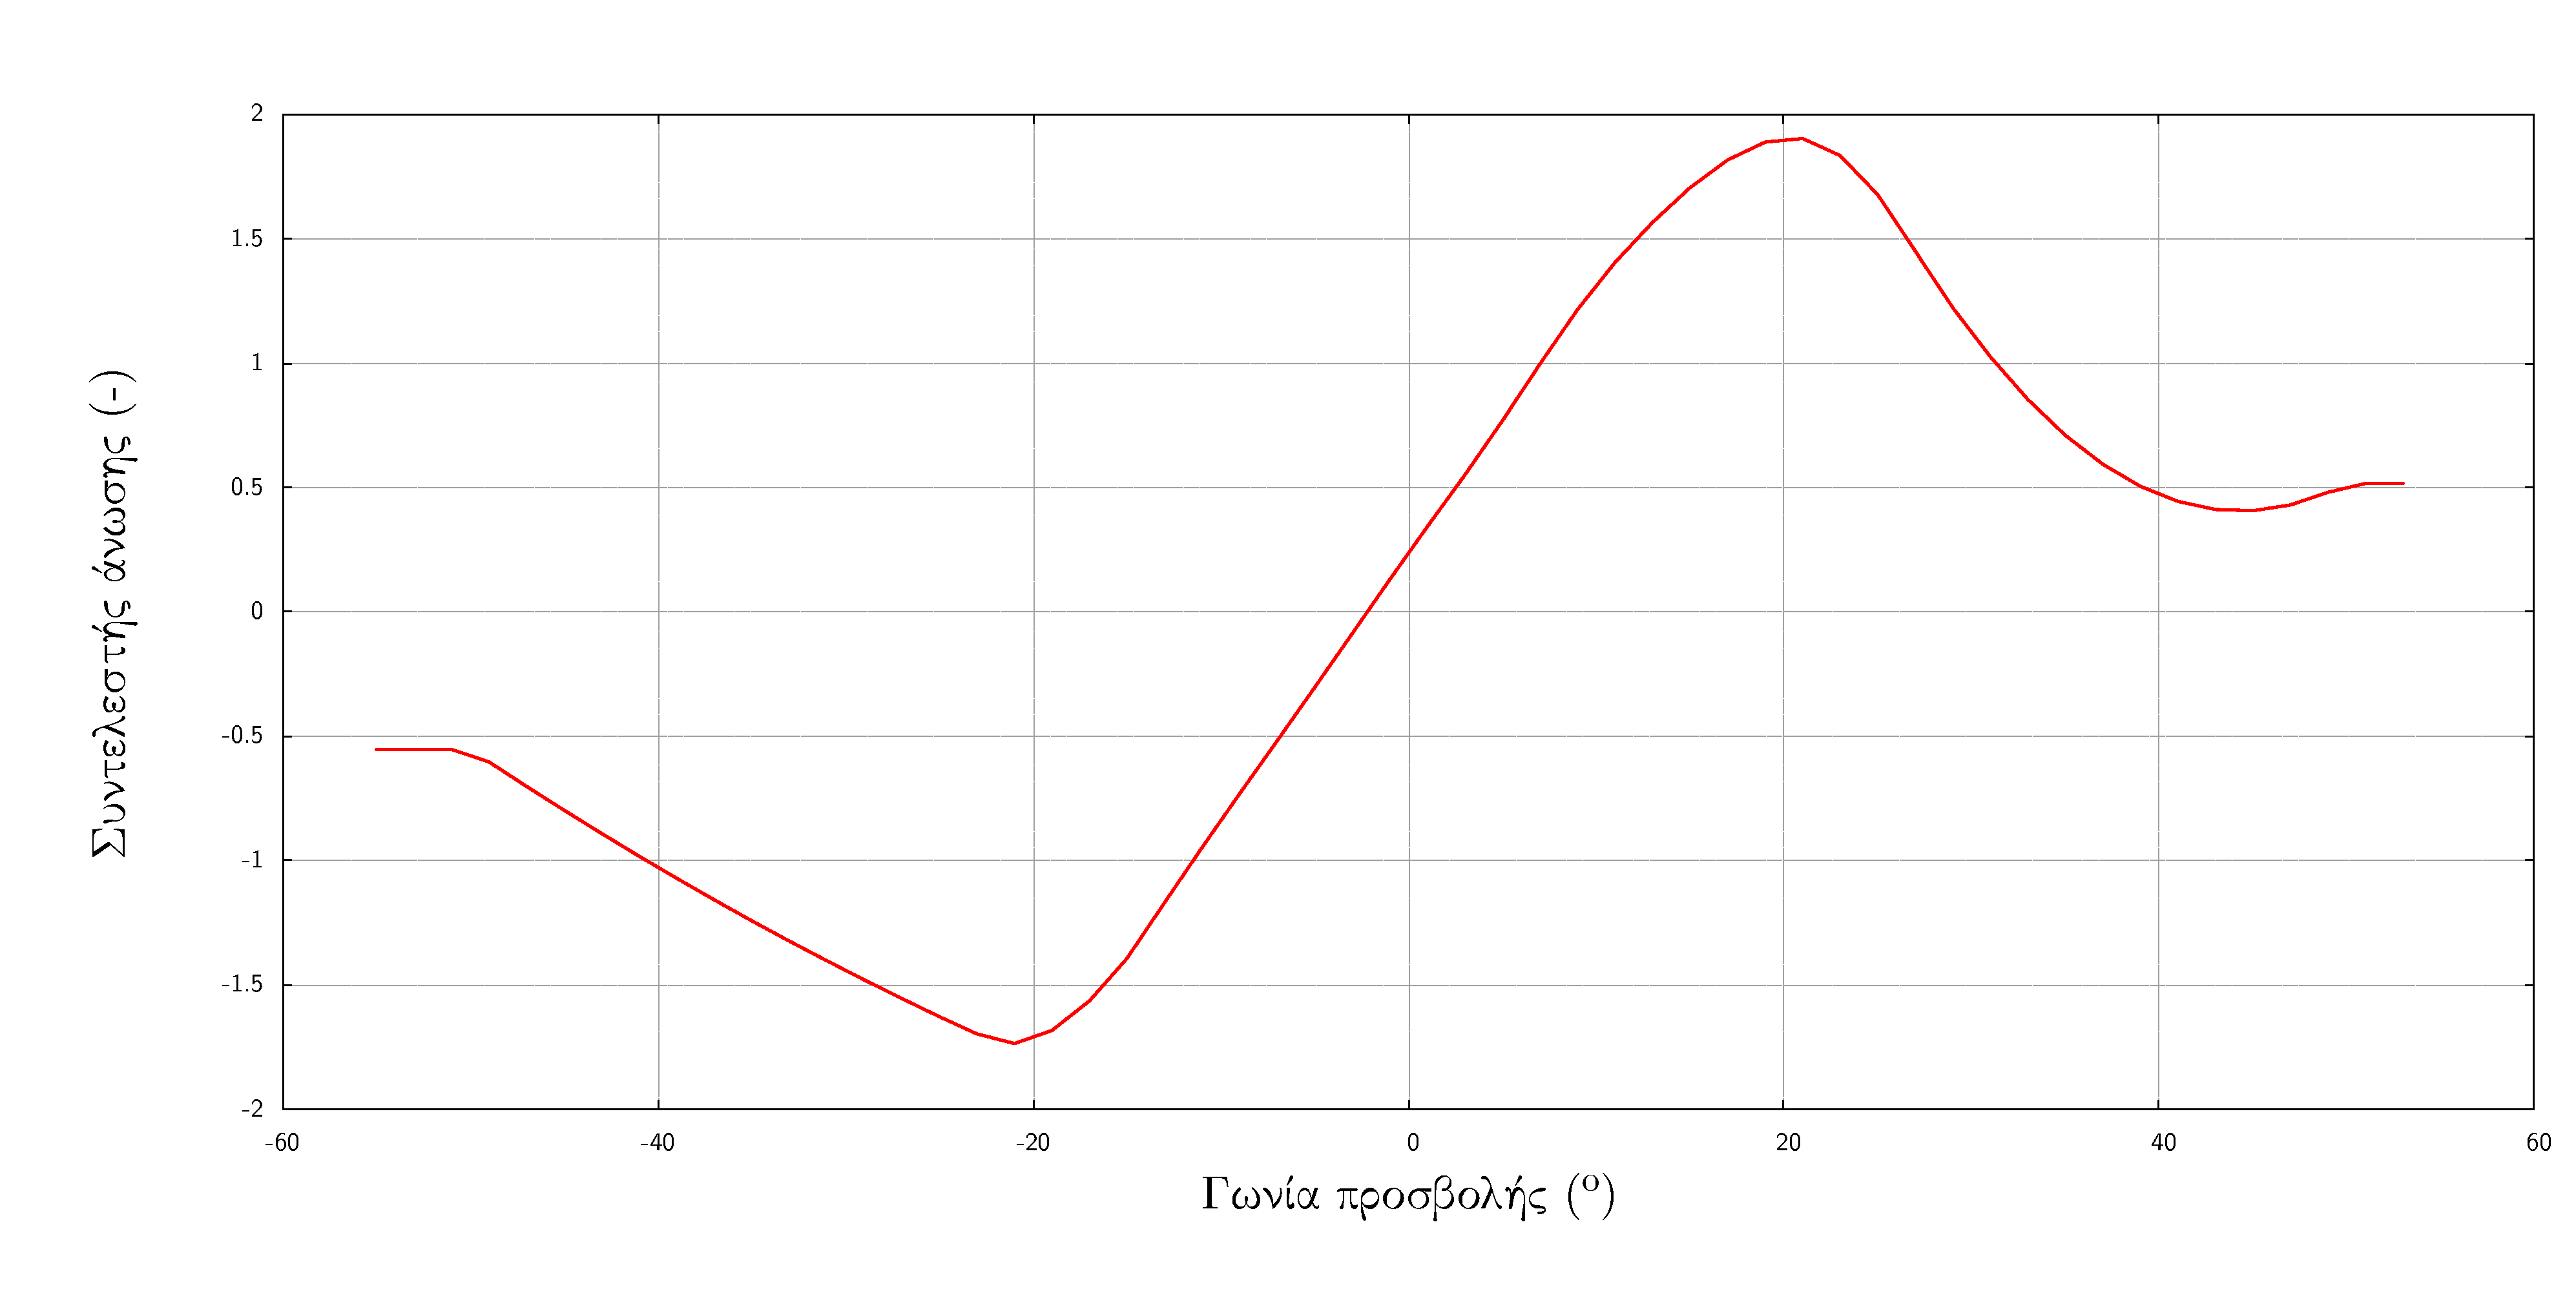
\includegraphics[width=0.85\textwidth]{figures/cl.pdf}
    \end{center}
    \caption{Διάγραμμα συντελεστή άνωσης}
    \label{fig:cl}
\end{figure}

\begin{figure}[ht!]
    \begin{center}
        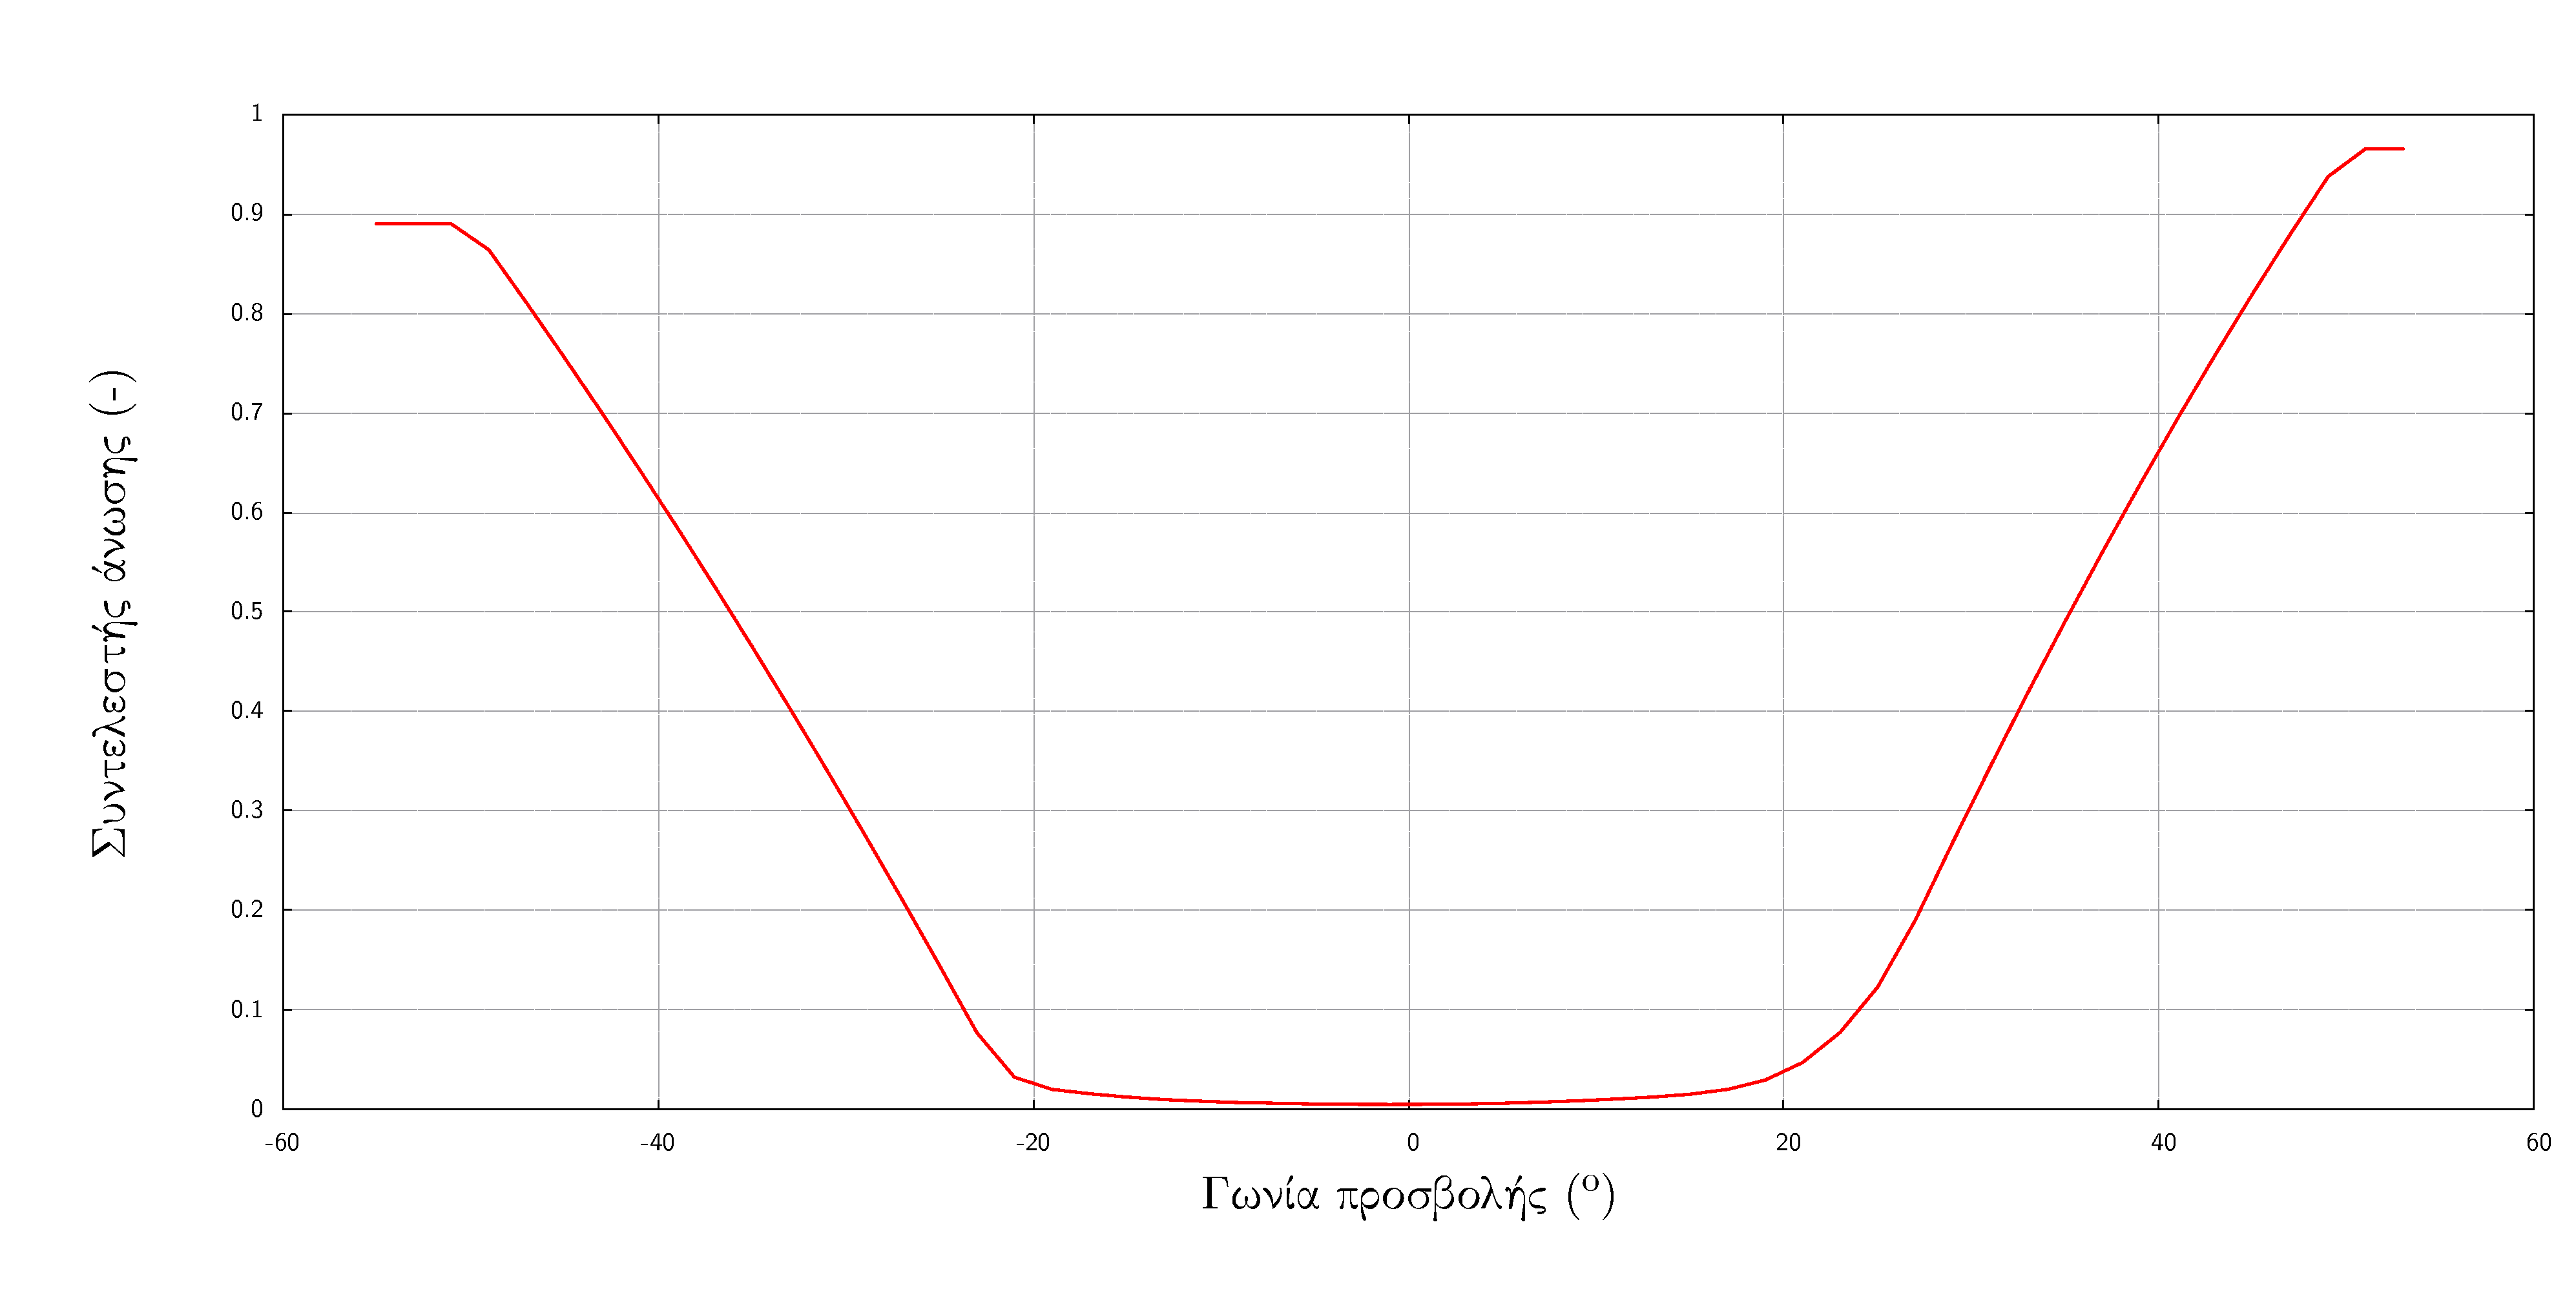
\includegraphics[width=0.85\textwidth]{figures/cd.pdf}
    \end{center}
    \caption{Διάγραμμα συντελεστή αντίστασης}
    \label{fig:cd}
\end{figure}

Με δεδομένες καμπύλες των αεροδυναμικών συντελεστών, μπορούμε να υπολογίσουμε τα αεροδυναμικά φορτία. Αρχικά, πρέπει να ορίσουμε τη φαινομενική ταχύτητα της ροής και τη φαινομενική γωνία προσβολής και η έκφρασή τους λαμβάνωντας υπόψη την κίνηση της αεροτομής δίνεται παρακάτω.

\begin{align}
   W_{eff} &= \sqrt{\big(-Wcos(\theta+\alpha)-\dot{u}\big)^2 + \big(Wsin(\theta+\alpha)-\dot{w})^2}\\[6pt]\label{eq:weff}
   \alpha_{eff} &= -atan\Big(\dfrac{Wsin(\alpha + \theta)-\dot{w}}{-Wcos(\alpha+\theta)-\dot{u}}\Big) - \theta\label{eq:aeff}
\end{align}

Και επομένως, κατά τα γνωστά, η δύναμη αντίστασης και άνωσης δίνονται απο τη σχέση \ref{eq:liftDrag}, και μετασχηματισμένες στο γενικό σύστημα απο τη σχέση \ref{eq:loads}.

\begin{equation}
    \begin{aligned}
    L &= \dfrac{1}{2}\rho\cdot c \cdot C_L(\alpha_{eff}) \cdot W_{eff}^2 \\
    D &= \dfrac{1}{2}\rho\cdot c \cdot C_D(\alpha_{eff}) \cdot W_{eff}^2 
    \end{aligned}
    \label{eq:liftDrag}
\end{equation}

\begin{equation}
    \begin{aligned}
    F_x &= L\cdot sin(\alpha_{eff}+\theta)-D \cdot cos(\alpha_{eff}+\theta) \\[5pt]
    F_z &= L\cdot cos(\alpha_{eff}+\theta)+D \cdot sin(\alpha_{eff}+\theta)
    \end{aligned}
    \label{eq:loads}
\end{equation}

\vspace{0.5cm}

\noindent Επομένως, πλεόν, παραγωγίζωντας τις σχέσεις \ref{eq:loads} μπορούμε να λάβουμε το μητρώο της αεροδυναμικής απόσβεσης, όπως προκύπτει απο την εξίσωση \ref{eq:linAeroel}. 

\vspace{0.5cm}

\begin{equation}
    \begin{aligned} 
    \dpart{F_x}{\dot{u}} &= \dpart{L}{\dot{u}}\cdot sin(\alpha_{eff}+\theta) + L \cdot cos(\alpha_{eff}+\theta})\cdot \dpart{\alpha_{eff}}{\dot{u}}\\
    &-\dpart{D}{\dot{u}}\cdot cos(\alpha_{eff}+\theta) + D\cdot sin(\alpha_{eff}+\theta)\cdot\dpart{\alpha_{eff}}{\dot{u}}
    \end{aligned} 
    \label{eq:partFxu}
\end{equation}

\vspace{0.8cm}

\begin{equation}
    \begin{aligned} 
    \dpart{F_x}{\dot{w}} &= \dpart{L}{\dot{w}}\cdot sin(\alpha_{eff}+\theta) + L \cdot cos(\alpha_{eff}+\theta})\cdot \dpart{\alpha_{eff}}{\dot{w}}\\
    &-\dpart{D}{\dot{w}}\cdot cos(\alpha_{eff}+\theta) + D\cdot sin(\alpha_{eff}+\theta)\cdot\dpart{\alpha_{eff}}{\dot{w}}
    \end{aligned} 
    \label{eq:partFxw}
\end{equation}

\vspace{0.5cm}

Και αντίστοιχα για την $F_z$.

\vspace{0.5cm}

\begin{equation}
    \begin{aligned} 
    \dpart{F_z}{\dot{u}} &= \dpart{L}{\dot{u}}\cdot cos(\alpha_{eff}+\theta) - L \cdot sin(\alpha_{eff}+\theta})\cdot \dpart{\alpha_{eff}}{\dot{u}}\\
    &+\dpart{D}{\dot{u}}\cdot sin(\alpha_{eff}+\theta) + D\cdot cos(\alpha_{eff}+\theta)\cdot\dpart{\alpha_{eff}}{\dot{u}}
    \end{aligned} 
    \label{eq:partFzu}
\end{equation}

\vspace{0.8cm}
\begin{equation}
    \begin{aligned} 
    \dpart{F_z}{\dot{w}} &= \dpart{L}{\dot{w}}\cdot cos(\alpha_{eff}+\theta) - L \cdot sin(\alpha_{eff}+\theta})\cdot \dpart{\alpha_{eff}}{\dot{w}}\\
    &+\dpart{D}{\dot{w}}\cdot sin(\alpha_{eff}+\theta) + D\cdot cos(\alpha_{eff}+\theta)\cdot\dpart{\alpha_{eff}}{\dot{w}}
    \end{aligned} 
    \label{eq:partFzw}
\end{equation}

\vspace{0.5cm}

Για τον υπολογισμό των παραγώγων απο τις \crefrange{eq:partFxu}{eq:partFzw}, χρειαζόμαστε τις εκφράσεις των $\dpart{L}{\dot{\mathbf{u}}}, \dpart{D}{\dot{\mathbf{u}}}, \dpart{\alpha_{eff}}{\dot{\mathbf{u}}}$. Θεωρώντας πως $W_{eff}\approx W$, οι παραπάνω παράγωγοι είναι.

\begin{equation}
   \begin{aligned} 
   \dpart{L}{\dot{u}} &= \dpart{C_L}{\dot{u}}\cdot\dfrac{\rho}{2}\cdot c \cdot W_{eff}^2 =\underline{ \dpart{C_L}{\alpha_{eff}}\cdot \dpart{\alpha_{eff}}{\dot{u}}\cdot\dfrac{\rho}{2}\cdot c \cdot W_{eff}^2}\\[8pt]
   \dpart{L}{\dot{w}} &= \dpart{C_L}{\dot{w}}\cdot\dfrac{\rho}{2}\cdot c \cdot W_{eff}^2 =\underline{ \dpart{C_L}{\alpha_{eff}}\cdot \dpart{\alpha_{eff}}{\dot{w}}\cdot\dfrac{\rho}{2}\cdot c \cdot W_{eff}^2}\\
   \end{aligned} 
    \label{eq:partL}
\end{equation}

\vspace{0.8cm}

\begin{equation}
   \begin{aligned} 
   \dpart{D}{\dot{u}} &= \dpart{C_D}{\dot{u}}\cdot\dfrac{\rho}{2}\cdot c \cdot W_{eff}^2 =\underline{ \dpart{C_D}{\alpha_{eff}}\cdot \dpart{\alpha_{eff}}{\dot{u}}\cdot\dfrac{\rho}{2}\cdot c \cdot W_{eff}^2}\\[8pt]
   \dpart{D}{\dot{w}} &= \dpart{C_D}{\dot{w}}\cdot\dfrac{\rho}{2}\cdot c \cdot W_{eff}^2 =\underline{ \dpart{C_D}{\alpha_{eff}}\cdot \dpart{\alpha_{eff}}{\dot{w}}\cdot\dfrac{\rho}{2}\cdot c \cdot W_{eff}^2}\\
   \end{aligned} 
    \label{eq:partD}
\end{equation}

\vspace{0.8cm}

\noindent Και απο την \cref{eq:aeff} η παράγωγοι $\dpart{\alpha_{eff}}{\dot{\mathbf{u}}}$ είναι.

\begin{align}
\dpart{\alpha_{eff}}{\dot{u}} &= \dfrac{-(Wsin(\alpha+\theta)-\dot{w})}{W^2 + \dot{u}^2 + \dot{w}^2 + 2\cdot W\cdot \dot{u} cos(\alpha+\theta) - 2\cdot W \cdot \dot{w} \cdot sin(\alpha+\theta)}\\[8pt]
\dpart{\alpha_{eff}}{\dot{w}} &= \dfrac{-(W\cdot cos(\alpha+\theta)+\dot{u})}{W^2 + \dot{u}^2 + \dot{w}^2 + 2\cdot W\cdot \dot{u} cos(\alpha+\theta) - 2\cdot W \cdot \dot{w} \cdot sin(\alpha+\theta)}
\label{eq:partAeff}
\end{align}

\vspace{0.8cm}

Αντικαθιστώντας τις \crefrange{eq:partL}{eq:partAeff} στις \crefrange{eq:partFxu}{eq:partFzw}, προκύπτουν οι τελικές εκφράσεις του μητρώου αεροδυναμικής απόσβεσης.

\begin{equation}
   \begin{aligned} 
   \dpart{F_x}{\dot{u}} = \dfrac{\rho}{2}\cdot W^2 \cdot c \cdot \dpart{\alpha_{eff}}{\dot{u}} \cdot & \Bigg[sin(\alpha_{eff}+\theta)\Big(\dpart{C_L}{\alpha_{eff}}+C_D\Big) + \\
   &+ cos(\alpha_{eff}+\theta)\Big(C_L-\dpart{C_D}{\alpha_{eff}}\Big)\Bigg]
   \end{aligned} 
    \label{eq:Fxu}
\end{equation}

\begin{equation}
   \begin{aligned} 
   \dpart{F_x}{\dot{w}} = \dfrac{\rho}{2}\cdot W^2 \cdot c \cdot \dpart{\alpha_{eff}}{\dot{w}} \cdot & \Bigg[sin(\alpha_{eff}+\theta)\Big(\dpart{C_L}{\alpha_{eff}}+C_D\Big) + \\
   &+ cos(\alpha_{eff}+\theta)\Big(C_L-\dpart{C_D}{\alpha_{eff}}\Big)\Bigg]
   \end{aligned} 
    \label{eq:Fxw}
\end{equation}

\vspace{0.6cm}

\begin{equation}
   \begin{aligned} 
   \dpart{F_z}{\dot{u}} = \dfrac{\rho}{2}\cdot W^2 \cdot c \cdot \dpart{\alpha_{eff}}{\dot{u}} \cdot & \Bigg[sin(\alpha_{eff}+\theta)\Big(\dpart{C_D}{\alpha_{eff}}+C_L\Big) + \\
   &+ cos(\alpha_{eff}+\theta)\Big(C_D-\dpart{C_L}{\alpha_{eff}}\Big)\Bigg]
   \end{aligned} 
    \label{eq:Fzu}
\end{equation}

\begin{equation}
   \begin{aligned} 
   \dpart{F_z}{\dot{w}} = \dfrac{\rho}{2}\cdot W^2 \cdot c \cdot \dpart{\alpha_{eff}}{\dot{w}} \cdot & \Bigg[sin(\alpha_{eff}+\theta)\Big(\dpart{C_D}{\alpha_{eff}}+C_L\Big) + \\
   &+ cos(\alpha_{eff}+\theta)\Big(C_D-\dpart{C_L}{\alpha_{eff}}\Big)\Bigg]
   \end{aligned} 
    \label{eq:Fzw}
\end{equation}

\noindent Και τελικά

\begin{equation}
    [\mathbf{C}] = 
    \begin{bmatrix}
        -\dpart{F_x}{\dot{u}} & -\dpart{F_x}{\dot{w}}\\[10pt]
        -\dpart{F_z}{\dot{u}} & -\dpart{F_z}{\dot{w}}\\
    \end{bmatrix}
    \label{eq:steadyC}
\end{equation}

\subsection{Αεροελαστικές εξισώσεις μη-μόνιμης ροής}

Για τη διατύπωση των αεροελαστικών εξισώσεων μη-μόνιμης ροής, χρησιμοποιούμε τη διατύπωση των αεροδυναμικών φορτίων που παρέχουν οι εξισώσεις του Theodorsen για προσκολλημένη ροή. Οι εξισώσεις του Theodorsen, προσεγγίζουν την αεροτομή ως μια διδιάστατη επιφάνεια (επίπεδη πλάκα χωρίς πάχος), και θεωρούν πως η αεροδυναμική συμπεριφορά της αεροτομής κυριαρχείται απο την κίνησή της κάθετα στην χορδή της. Στην τελική διατύπωση τους, οι εξισώσεις του Theodorsen λαμβάνουν υπόψη την επίδραση του ομόρρου στο οριακό στρώμα της πτέρυγας και επιπλέον συνυπολογίζουν την προστιθέμενη μάζα που προκύπτει απο το ρευστό λόγω της επιτάχυνσης της πτέρυγας (κάθετα στην χορδή). Οι εξισώσεις του Theodorsen στην αρχική τους μορφή, θεωρούν και στροφικό βαθμό ελευθερίας της πτέρυγας, ωστόσο ακολουθώντας τις αρχικές θεωρήσεις μας, όλοι οι αντίστοιχοι όροι έχουν μηδενισθεί. Η έκφραση του συντελεστή άνωσης απο τις εξισώσεις του Theodorsen παρουσιάζεται στην \cref{eq:theodorsen}.

\begin{equation}
    C_L = 2\pi \Big(\alpha_{E}(t)-\alpha_0\Big) - \underbrace{\dfrac{\pi\cdot c\cdot \ddot{h}}{2\cdot W_{eff}^2}}_{\text{Όρος προστιθέμενης μάζας}}
    \label{eq:theodorsen}
\end{equation}

\noindent Όπου $\ddot{\mathbf{h}}=\ddot{w}cos\theta+\ddot{u}sin\theta$ η επιτάχυνση της πτέρυγας κάθετα στη χορδή.
Σημειώνεται πως για αύξηση της ακρίβειας, ο συντελεστής $2\pi$ μπορεί να αντικατασταθεί απο την κλίση της καμπύλης $C_L\text{--}\alpha$ στη γραμμική περιοχή, δηλαδή $\dfrac{dC_L}{d\alpha}\Bigg|_{\text{γραμμ}}$

\vspace{0.5cm}

Επιπλέον, λόγω της φαινόμενης γωνίας προσβολής, επάγεται αντίσταση στο σύστημα παράλληλο με τη χορδή, και ο συντελεστής αντίστασης είναι

\begin{equation}
    C_D = C_{D,\text{μον}}(\alpha_{E}) + C_L\cdot (\alpha_{eff}-\alpha_E)
\end{equation}

\noindent Η φαινόμενη γωνία προσβολής ($\alpha_E$) είναι ο όρος που λαμβάνει υπόψη την επίδραση του ομόρρου στο οριακό στρώμα της αεροτομής και συχνά καλείται όρος ανακυκλοφορίας. Αναπτύσσωντας την ποσότητα $\alpha_E$ έχουμε:

\begin{equation}
    \alpha_E = C(k)\alpha_{eff}
    \label{eq:ae}
\end{equation}

\noindent
Με

\begin{equation}
\alpha_{eff} = \alpha - \theta -\dfrac{\dot{h}}{W_{eff}^2}
    \label{eq:aeff_uns}
\end{equation}


\noindent
Όπου, $C(k)$ αποκαλούμε τη συνάρτηση Theodorsen, που συσχετίζει την ταλάντωση του πεδίου ροής στον ομόρρου με την πίεση στην επιφάνεια της αεροτομής, δηλαδή ποσοτικοποιεί την επίδραση της ταλάντωσης στον ομόρρου στον συντελεστή άνωσης. 

Καθώς ο υπολογισμός της συνάρτησης Theodorsen είναι αρκετά επίπονος, θα υπολογίσουμε την φαινόμενη γωνία προσβολής $\alpha_E$ απο την \cref{eq:ae_diff}, όπου $y_1, y_2$ δύο επιπλέον αεροδυναμικοί βαθμοί ελευθερίας, που προκύπτουν απο τη λύση του συστήματος Σ.Δ.Ε \ref{eq:aeroode}.

\begin{equation}
    \alpha_{E} = \alpha_{eff}\cdot (1-A_1-A_2)+y_1+y_2
    \label{eq:ae_diff}
\end{equation}

\begin{equation}
    \begin{aligned}
        \dot{y_1} + b_1\dfrac{2W_{eff}}{c}y_1-b_1A_1\dfrac{2W_{eff}}{c}\alpha_{eff} &=0\\
        \dot{y_2} + b_2\dfrac{2W_{eff}}{c}y_2-b_2A_2\dfrac{2W_{eff}}{c}\alpha_{eff} &=0\\
    \end{aligned}
    \label{eq:aeroode}
\end{equation}

\noindent Με $A_1=0.165$, $A_2=0.335$, $b_1=0.0455$, $b_2=0.3000$.

\vspace{0.5cm}

Ως οριακές συνθήκες των εξισώσεων \ref{eq:aeroode} ορίζουμε πως για $t=0$ έχουμε $\alpha_{E}=\alpha_{eff}$ οπότε προκύπτει $y_1(0) = A_1\alpha_{eff}$ και $y_2(0) = A_2\alpha_{eff}$. Οι εξισώσεις \ref{eq:aeroode} διακριτοποιούνται με πεπερασμένες διαφορές και υπολογίζουμε τις τιμές των $y_1,y_2$ πριν τον υπολογισμό των εξωτερικών φορτίων από την \cref{eq:loads}.

Για να υπολογίσουμε πλέον, τις παραγώγους των αεροδυναμικών φορτίων και συνεπώς το μητρώο αεροδυναμικής απόσβεσης διαφορίζουμε τις Δ.Ε \ref{eq:aeroode}.

\begin{equation}
    \dpart{}{\dot{u}}\Big(\dfrac{dy_1}{dt}\Big) + b_1\dfrac{2W_{eff}}{c}\dpart{y_1}{\dot{u}}-b_1A_1\dfrac{2W_{eff}}{c}\dpart{\alpha_{eff}}{\dot{u}} = 0
    \label{eq:diffOde}
\end{equation}

Θεωρώντας τον όρο δεύτερης τάξης $\dpart{}{\dot{u}}\Big(\dfrac{dy_1}{dt}\Big) \approx 0$ προκύπτει:

\begin{align}
    \dpart{y_1}{\dot{\mathbf{u}}}&=A_1\dpart{\alpha_{eff}}{\dot{\mathbf{u}}}\label{eq:y1der}\\[10pt]
    \dpart{y_2}{\dot{\mathbf{u}}}&=A_2\dpart{\alpha_{eff}}{\dot{\mathbf{u}}}\label{eq:y2der}
\end{align}

Επιπλέον,

\begin{equation}
    \dpart{\alpha_E}{\dot{\mathbf{u}}} = (1-A_1-A_2)\dpart{\alpha_{eff}}{\dot{\mathbf{u}}} + \dpart{y_1}{\dot{\mathbf{u}}} + \dpart{y_2}{\dot{\mathbf{u}}}
    \label{eq:aeder}
\end{equation}

Και αντικαθιστώντας τις \crefrange{eq:y1der}{eq:y2der}, προκύπτει:

\begin{equation}
    \dpart{\alpha_E}{\dot{\mathbf{u}}} = \dpart{\alpha_{eff}}{\dot{\mathbf{u}}}
\end{equation}

Ενώ απο την \cref{eq:aeff_uns} είναι:

\begin{equation}
    \begin{aligned}
        \dpart{\alpha_{eff}}{\dot{u}} = -sin(\theta)\\[6pt]
        \dpart{\alpha_{eff}}{\dot{w}} = -cos(\theta)
    \end{aligned}
\end{equation}

Επομένως, τελικά έχουμε

\begin{equation}
    \dpart{C_L}{\dot{\mathbf{u}}} = \dfrac{dC_L}{d\alpha}\Bigg|_{\text{γραμμ}} \cdot \dpart{\alpha_{eff}}{\dot{\mathbf{u}}}
\end{equation}

Και για τον συντελεστή αντίστασης 

\begin{equation}
    \dpart{C_D}{\dot{\mathbf{u}}} = \dpart{C_D}{\alpha}\cdot\dpart{\alpha_{eff}}{\dot{\mathbf{u}}} + \dpart{C_L}{\dot{\mathbf{u}}}\cdot(\alpha_{eff}-\alpha_E)
\end{equation}

Και οι τελικές τιμές των παραγώγων των αεροδυναμικών φορτίων υπολογίζονται απο τις \crefrange{eq:partFxu}{eq:partD}. Σημειώνεται ωστόσο, πως η θεώρηση του όρου $\dpart{}{\dot{u}}\Big(\dfrac{dy_1}{dt}\Big) \approx 0$ αγνοεί την επιρροή του ομόρρου στην αεροδυναμική απόσβεση της αεροτομής και αποτελεί μια παραδοχή για απλοποίηση των υπολογισμών και την αποφυγή της επίλυσης μιας ακόμη Σ.Δ.Ε. Ωστόσο, όπως θα δούμε και σε επόμενη παράγραφο, αν δεν λύσουμε την γραμμικοποιημένη εξίσωση για τον προσδιορισμό της χρονοσειράς των αποκρίσεων, αλλά χρησιμοποιήσουμε την αρχική έκφραση, αυτή η απλοποίηση δεν αποτελεί αίτιο προβληματισμού. Ωστόσο, αν θέλαμε να συγκρίνουμε τις τιμές της απόσβεσης που δίνουν οι εκφράσεις των μόνιμων και μη-μόνιμων μοντέλων, θα ήταν αναγκαίο να συμπεριλάβουμε και τον όρο δεύτερης τάξης. 
